% This file was created with tikzplotlib v0.10.1.
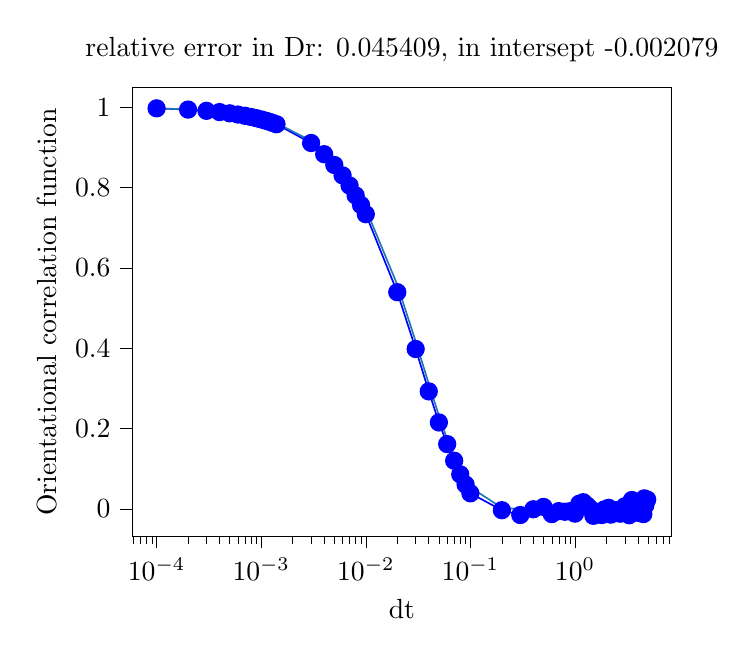
\begin{tikzpicture}

\definecolor{darkgray176}{RGB}{176,176,176}
\definecolor{steelblue31119180}{RGB}{31,119,180}

\begin{axis}[
log basis x={10},
tick align=outside,
tick pos=left,
title={relative error in Dr: 0.045409, in intersept -0.002079},
x grid style={darkgray176},
xlabel={dt},
xmin=5.8276061909058e-05, xmax=8.40825519000689,
xmode=log,
xtick style={color=black},
y grid style={darkgray176},
ylabel={Orientational correlation function},
ymin=-0.0674775242017615, ymax=1.04778267118092,
ytick style={color=black}
]
\addplot [semithick, blue, mark=*, mark size=3, mark options={solid}]
table {%
0.0001 0.996869693545155
0.0002 0.99375059517542
0.0003 0.990648067986859
0.0004 0.987559120179877
0.0005 0.984484804565178
0.0006 0.98142440500064
0.0007 0.978373415925511
0.0008 0.97533123304194
0.0009 0.972301613836282
0.001 0.969284244964818
0.0011 0.966270397132582
0.0012 0.963267704178874
0.0013 0.960273485472013
0.0014 0.957279600974741
0.003 0.910618621274516
0.004 0.882786995930577
0.005 0.855984560313007
0.006 0.830090716897699
0.007 0.804783134950063
0.008 0.780215354996441
0.009 0.756510218433562
0.01 0.733608597868947
0.02 0.539512636985607
0.03 0.398183942634577
0.04 0.292817678536253
0.05 0.215491967276188
0.06 0.161659961969078
0.07 0.120236813652895
0.08 0.0864543024771473
0.09 0.0609180847676959
0.1 0.0392763923453196
0.2 -0.00282482229585726
0.3 -0.0148360605970169
0.4 -0.000489055092350534
0.5 0.00534602877754693
0.6 -0.0125123931031095
0.7 -0.00507160411676941
0.8 -0.0066307474648018
0.9 -0.00506955863390187
1 -0.0113321122049235
1.1 0.013294974964752
1.2 0.0170494922050192
1.3 0.00913424619466545
1.4 0.000927730467969378
1.5 -0.0167838789570943
1.6 -0.00981594409218104
1.7 -0.00745025920879478
1.8 -0.0148531907332654
1.9 -0.00135551050561144
2 0.00038612979905702
2.1 0.00307850208718369
2.2 -0.0138170476213894
2.3 -0.00283744677311507
2.4 -0.00792766216376212
2.5 -0.00751774768459342
2.6 -0.00175442753027426
2.7 -0.0114917026719802
2.8 -0.00493744910855643
2.9 -0.000664065265267109
3 0.00705980472571119
3.1 -0.0041364348774039
3.2 0.00268026972386246
3.3 -0.0152625491893497
3.4 0.00966372359702818
3.5 0.0225274335147701
3.6 -0.00842334747212409
3.7 0.00196390149066858
3.8 -0.00193245255738107
3.9 -0.00656658319262957
4 -0.00914694318526399
4.1 0.00856952775668718
4.2 0.00203322496745541
4.3 0.00540117085980913
4.4 -0.00635525274573205
4.5 -0.0125112297957199
4.6 0.0265895508806755
4.7 0.00892382779312095
4.8 0.0203085013691108
4.9 0.0236685940651423
};
\addplot [semithick, steelblue31119180]
table {%
0.0001 0.997089025936249
0.0002 0.994186525642498
0.0003 0.991292474451822
0.0004 0.988406847769101
0.0005 0.985529621070811
0.0006 0.982660769904815
0.0007 0.979800269890157
0.0008 0.97694809671685
0.0009 0.974104226145677
0.001 0.971268634007976
0.0011 0.968441296205444
0.0012 0.965622188709925
0.0013 0.962811287563207
0.0014 0.960008568876824
0.003 0.916258658703931
0.004 0.889933295837348
0.005 0.864364296606157
0.006 0.839529929649928
0.007 0.815409087979898
0.008 0.791981271039925
0.009 0.769226567282849
0.01 0.747125637247457
0.02 0.558196717832419
0.03 0.417043078519985
0.04 0.311583575798885
0.05 0.232792077624583
0.06 0.173924929341426
0.07 0.129943773667432
0.08 0.0970843247076193
0.09 0.0725341879639191
0.1 0.0541921514047699
0.2 0.0029367892738775
0.3 0.000159150928973874
0.4 8.62473123916195e-06
0.5 4.67392741138113e-07
0.6 2.53290181932471e-08
0.7 1.37263398886261e-09
0.8 7.4385988947776e-11
0.9 4.03113677545142e-12
1 2.18455974468599e-13
1.1 1.18385992436788e-14
1.2 6.41559162633841e-16
1.3 3.47674712765705e-17
1.4 1.88412406738089e-18
1.5 1.02104736724876e-19
1.6 5.53327535173865e-21
1.7 2.99860095625702e-22
1.8 1.62500637023969e-23
1.9 8.80625912497442e-25
2 4.77230127810253e-26
2.1 2.58621273412109e-27
2.2 1.40152432052433e-28
2.3 7.59516181753216e-30
2.4 4.11598159159435e-31
2.5 2.23053897590927e-32
2.6 1.20877705896715e-33
2.7 6.55062293941603e-35
2.8 3.54992350128392e-36
2.9 1.92377991856926e-37
3 1.04253772616563e-38
3.1 5.64973623015521e-40
3.2 3.06171361181585e-41
3.3 1.65920847609569e-42
3.4 8.99160769486551e-44
3.5 4.87274565572452e-45
3.6 2.64064570331958e-46
3.7 1.43102271760647e-47
3.8 7.75501997761952e-49
3.9 4.20261216774172e-50
4 2.2774859488979e-51
4.1 1.23421863364909e-52
4.2 6.68849630613008e-54
4.3 3.6246400449205e-55
4.4 1.96427042102118e-56
4.5 1.06448040055892e-57
4.6 5.76864830344984e-59
4.7 3.12615462261427e-60
4.8 1.69413044623436e-61
4.9 9.18085736417613e-63
};
\end{axis}

\end{tikzpicture}
